

% Gradient Info
  
\tikzset {_geld2178i/.code = {\pgfsetadditionalshadetransform{ \pgftransformshift{\pgfpoint{0 bp } { 0 bp }  }  \pgftransformrotate{0 }  \pgftransformscale{2 }  }}}
\pgfdeclarehorizontalshading{_8gtsa1tg3}{150bp}{rgb(0bp)=(1,1,1);
rgb(37.5bp)=(1,1,1);
rgb(48.48214285714286bp)=(0.96,0.65,0.14);
rgb(100bp)=(0.96,0.65,0.14)}
\tikzset{every picture/.style={line width=0.75pt}} %set default line width to 0.75pt        

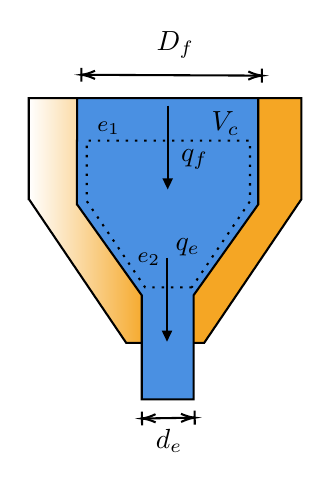
\begin{tikzpicture}[x=0.75pt,y=0.75pt,yscale=-1,xscale=1]
%uncomment if require: \path (0,300); %set diagram left start at 0, and has height of 300

%Shape: Path Data [id:dp9492299757340803] 
\path  [shading=_8gtsa1tg3,_geld2178i] (209.58,169.75) -- (172,169.75) -- (125.15,100.53) -- (125.04,100.53) -- (125.04,51.86) -- (256.43,51.86) -- (256.43,100.53) -- (209.58,169.75) -- cycle ; % for fading 
 \draw   (209.58,169.75) -- (172,169.75) -- (125.15,100.53) -- (125.04,100.53) -- (125.04,51.86) -- (256.43,51.86) -- (256.43,100.53) -- (209.58,169.75) -- cycle ; % for border 

%Shape: Path Data [id:dp15137488085975803] 
\draw  [fill={rgb, 255:red, 74; green, 144; blue, 226 }  ,fill opacity=1 ] (148.35,103.07) -- (148.28,103.07) -- (148.28,72.3) -- (148.33,72.3) -- (148.33,51.86) -- (235.61,51.86) -- (235.61,103.07) -- (204.47,146.83) -- (204.47,197) -- (179.49,197) -- (179.49,146.83) -- (148.35,103.07) -- cycle ;
%Straight Lines [id:da2754383415374976] 
\draw    (150.4,40.6) -- (237.4,41) ;
\draw [shift={(237.4,41)}, rotate = 180.26] [color={rgb, 255:red, 0; green, 0; blue, 0 }  ][line width=0.75]    (0,3.35) -- (0,-3.35)(6.56,-1.97) .. controls (4.17,-0.84) and (1.99,-0.18) .. (0,0) .. controls (1.99,0.18) and (4.17,0.84) .. (6.56,1.97)   ;
\draw [shift={(150.4,40.6)}, rotate = 0.26] [color={rgb, 255:red, 0; green, 0; blue, 0 }  ][line width=0.75]    (0,3.35) -- (0,-3.35)(6.56,-1.97) .. controls (4.17,-0.84) and (1.99,-0.18) .. (0,0) .. controls (1.99,0.18) and (4.17,0.84) .. (6.56,1.97)   ;
%Straight Lines [id:da2165549302677806] 
\draw    (179.6,206.2) -- (205,205.8) ;
\draw [shift={(205,205.8)}, rotate = 179.1] [color={rgb, 255:red, 0; green, 0; blue, 0 }  ][line width=0.75]    (0,3.35) -- (0,-3.35)(6.56,-1.97) .. controls (4.17,-0.84) and (1.99,-0.18) .. (0,0) .. controls (1.99,0.18) and (4.17,0.84) .. (6.56,1.97)   ;
\draw [shift={(179.6,206.2)}, rotate = 359.1] [color={rgb, 255:red, 0; green, 0; blue, 0 }  ][line width=0.75]    (0,3.35) -- (0,-3.35)(6.56,-1.97) .. controls (4.17,-0.84) and (1.99,-0.18) .. (0,0) .. controls (1.99,0.18) and (4.17,0.84) .. (6.56,1.97)   ;
%Shape: Path Data [id:dp5403946800956351] 
\draw  [dash pattern={on 0.84pt off 2.51pt}] (203.62,143) -- (181.11,143) -- (153.06,101.51) -- (153,101.51) -- (153,72.33) -- (231.67,72.33) -- (231.67,101.51) -- (203.62,143) -- cycle ;
%Straight Lines [id:da5188554524250316] 
\draw    (191.67,128.83) -- (191.67,166.17) ;
\draw [shift={(191.67,169.17)}, rotate = 270] [fill={rgb, 255:red, 0; green, 0; blue, 0 }  ][line width=0.08]  [draw opacity=0] (5.36,-2.57) -- (0,0) -- (5.36,2.57) -- cycle    ;
%Straight Lines [id:da22307227495117776] 
\draw    (192,55.5) -- (192,92.83) ;
\draw [shift={(192,95.83)}, rotate = 270] [fill={rgb, 255:red, 0; green, 0; blue, 0 }  ][line width=0.08]  [draw opacity=0] (5.36,-2.57) -- (0,0) -- (5.36,2.57) -- cycle    ;

% Text Node
\draw (185.2,18.4) node [anchor=north west][inner sep=0.75pt]   [align=left] {$\displaystyle D_{f}$};
% Text Node
\draw (184.8,209.8) node [anchor=north west][inner sep=0.75pt]   [align=left] {$\displaystyle d_{e}$};
% Text Node
\draw (197,75) node [anchor=north west][inner sep=0.75pt]   [align=left] {$\displaystyle q_{f}$};
% Text Node
\draw (194.33,118) node [anchor=north west][inner sep=0.75pt]   [align=left] {$\displaystyle q_{e}$};
% Text Node
\draw (156.67,62) node [anchor=north west][inner sep=0.75pt]  [font=\footnotesize] [align=left] {$\displaystyle e_{1}$};
% Text Node
\draw (176,125) node [anchor=north west][inner sep=0.75pt]  [font=\footnotesize] [align=left] {$\displaystyle e_{2}$};
% Text Node
\draw (211.67,57) node [anchor=north west][inner sep=0.75pt]   [align=left] {$\displaystyle V_{c}$};


\end{tikzpicture}
